When controlling the beam angle without any ball on the beam, we are using a simple PID controller. When controlling the ball position along the beam, we are instead using a cascaded PID controller setup (see figure \ref{fig:cascaded_pid}).
Our implementation also alows for an additional beam angle reference to be supplied as a feed forward signal if desired, but in our final setup we do note make use of this.
\begin{figure}
\centering
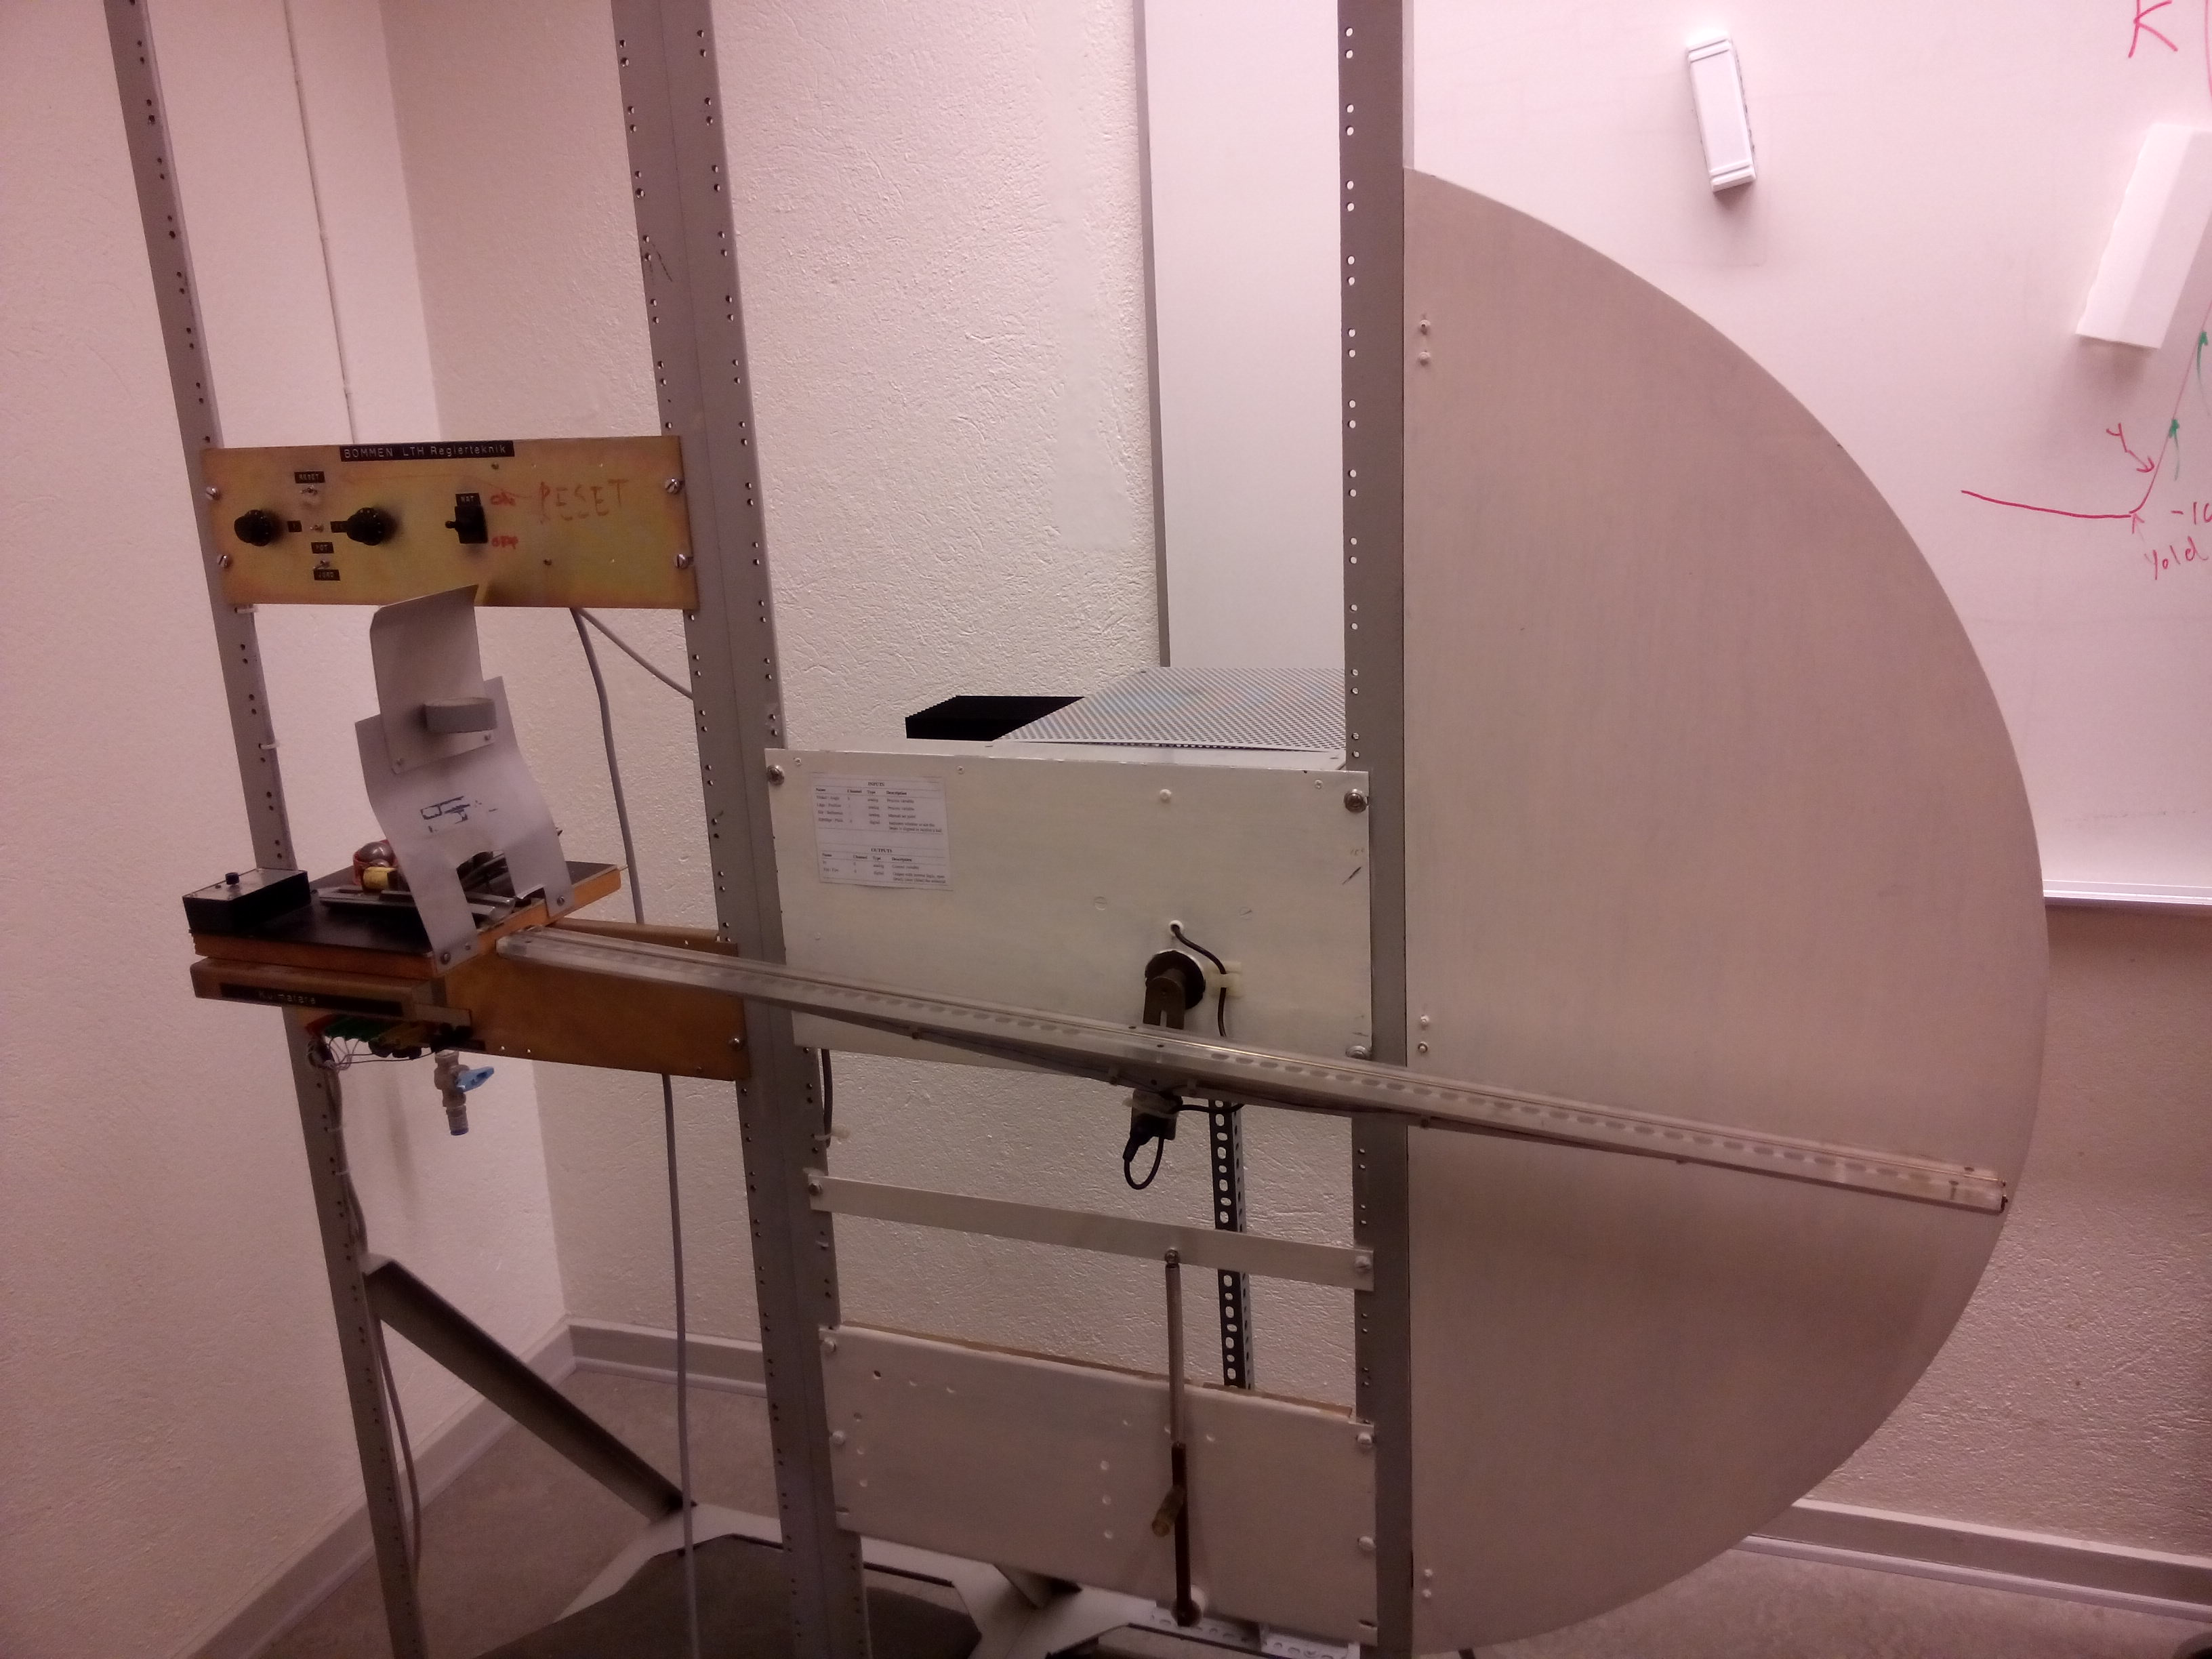
\includegraphics[width=0.7\textwidth]{figures/process_fig.jpg}
\caption{?????????????FIX BLOCK DIAGRAM???????????????The cascaded PID setup.}\label{fig:cascaded_pid}
\end{figure}

As mentioned in the introduction, we have a sequence of tasks to be performed, and each of these (catching, weighing and delivering the ball) will be described in further detail in the following sections.

\subsection{Ball catching}
The ball magazine shown to the left of the beam in figure \ref{fig:process} is equipped with a ball dispatcher solenoid, which can be controlled from our program.
For the ball to roll onto the beam however, the beam has to be aligned with the dispatcher.

Since the sensor measuring the beam angle is not very reliable, we make use of an additional optical sensor detecting when the beam is aligned with the dispatcher.
Starting at some underestimated angle near the dispatcher, the search for the correct beam angle is done by slowly increasing the beam angle until the optical sensor triggers. A small beam angle bias is then corrected for dispatching a ball.

\subsection{Ball weighing}
HIGH TOLERANCE HERE \\

\subsection{Ball delivery}

